%TEX root = ../dissertation.tex

\iffalse \bibliography{bibliography/dissertation} \fi

\chapter{Designing a Programming Environment for Generative Design}
\label{chapter:pegd}

\section{Design Principles} 

Programming is hard to learn. Unfortunately, as shown in the previous section, few programming languages or environments are designed to introduce the basics of good software engineering practice. Specially in Architecture, the environments used to support \gls{gd} either they are old or obsolete, or they enforce particular programming methods that are inadequate, or they are not pedagogic, meaning that they are not designed for the particular programming skills of the \gls{gd} community.

The literature is vast, but it is clearly divided in two perspectives: software engineering perspective, or psychological/educational perspective. That means either systems designed for expert programmers~\citep{carlson2005eclipse,intellij2001intellij,lighttable,boudreau2002netbeans,guckenheimer2006software}, or systems designed for novices~\citep{papert1980mindstorms,goldberg1983smalltalk,GuoSIGCSE2013,Reas2006}. The problem is that while programming systems designed for expert programmers are constantly updated, systems designed for novices are usually obsolete or in disuse. It negatively affects other communities that are not focused on develop software for industry, but for their own purpose which includes mainly novice users.

For example the \gls{gd} community is focused on build software to support Architecture methods, however designers are in desperate need of a programming system that correspond their needs. These needs are from different natures for instance: give support to the increasing adoption of \gls{gd} methods, deal with the increasingly complexity of current \gls{gd} programs, support tools that allows programs to be tested quicker, among others.

In the next section I propose...

\section{Program Documentation}

Program documentation is a software requirement of the utmost importance because it is a key factor for understanding programs. Even the best program, the most perfectly suitable for the job, will be essentially useless if the people who need to use it do not know what it is; cannot understand it well enough to use, build, or modify it; or (worst of all) misunderstand it and apply it incorrectly. And all of the effort, analysis, hard work, and insightful design spend to construct it will have been wasted.

Software exists for a specific reason and documentation exists to explain this reason. Every piece of code has its rational and a reason to be written in that way. Then the documentation recollects all these rationales organizing them in a form of different artifacts such as, requirements description, architectural models, data models, \gls{api} documentation, flow diagrams, use case diagrams, etc. So it is undoubtedly a rich source of information not only for the developer who did the software but also for the developer who will test the application, for the stakeholder who will use the application, and eventually for the developer who will maintain that code.

In fact software maintenance, traditionally defined as any modification made on a system after its delivery, is a dominant activity in software engineering. Some reports place maintenance at 90\% of the total cost of a typical software project~\citep{seacord2003modernizing,pigoski1996practical}. One of the main difficulties in software maintenance is a lack of up-to-date documentation~\citep{de2005study}. As a result, some studies indicate that 40\% to 60\% of maintenance activity is spent simply studying existing software~\citep[p. 475 and p. 35 respectively]{pigoski1996practical,pfleeger1998software}. Having an updated documentation would dramatically reduce the effort spent in this study, helping the developer to comprehend the code and maintain it.

The sad truth is that writing program documentation today is perceived as a tiresome task, if it is done at all, is often treated as an afterthought, something people do because they have to~\citep{sousa1998survey}. Bass et al. summarizes many possible reasons that lead programmers to write the documentation, and then concluded as follows:

\blockquote{Maybe a contract requires it. Maybe a customer demands it. Maybe a company's standard process calls for it. In fact, these may all be legitimate reasons. But none of them are compelling enough to produce high-quality documentation.~\citep[p. 327]{BassClementsKazman201210}}

Producing a high-quality documentation should be a natural developer's attitude not because it's ``required" but because they see that it is essential to the matter at hand. The documentation defends the developer's job because it speaks for him, for example in agile methods it can be used as contract~\citep{ambler2007agile}. It also helps developers reason about the architecture design of their programs, and communicate these ideas while the development is in progress. However produce useful documentation is a hard task and developers have to consider that some documentation artifacts are more important than others.

As described earlier, documentation is composed by several artifacts, formally defined as any artifact intended to communicate information on the software system~\citep{forward2002relevance}. This communication is aimed at human readers, from the technical document delivered to the developer team, until the user manual delivered to the users. But the central point from where the documentation comes from is the source code, as a result it is the most important artifact as confirmed in the following study:

\blockquote{Source code and comments are the most important artifact to understand a system to be maintained. Data model and requirement description were other important artifacts. Surprisingly, and contrary to what we found in the literature, architectural models and
other general view of the system are not very important. This could simply indicate that such documentation artifacts are used once to have a global understanding of the system and never consulted again after.~\citep[p. 74]{de2005study}}

The importance of source code and comments is a reality already noted in the software industry, so the use of automation tools to generate, verify, and maintain the source code documentation, is a common practice. The most frequently cited technologies, as concluded in~\citep{forward2002relevance}, are Javadoc\footnote{\texttt{http://docs.oracle.com/javase/7/docs/technotes/guides/javadoc/}} and DocWiz\footnote{\texttt{http://docwiz.sourceforge.net/}} to comment Java source code, Doc++\footnote{\texttt{http://docpp.sourceforge.net/}} and Doxygen\footnote{\texttt{http://www.stack.nl/dimitri/doxygen/index.html}} to comment source code in languages such as C, C++, and also Java. These tools generate an on-line documentation browser (in HTML) and/or an off-line reference manual (in $\mbox{\LaTeX}$) from a set of documented source files. The comments are inserted directly in the source code between a start tag and a end tag. These tags typically use the language's comment delimiter to prevent any compilation error, once the compiler will ignore any word between comments. In case of Javadoc an extra asterisk is needed to generate the documentation, so the comments are embed inside \texttt{/** ... */} (as shown in Figure~\ref{fig:javadoc-code}). Additionally, other tags are provided to document for example the function parameters (\texttt{@param}), the function return (\texttt{@return}), an exception that may be thrown from the method (\texttt{@exception}, \texttt{@throws}), and so on. As a result, these tags add proper information into the HTML page (e.g. as shown in Figure~\ref{fig:javadocgen}).

\begin{figure}
\centering
\begin{subfigure}{.5\textwidth}
  \centering
  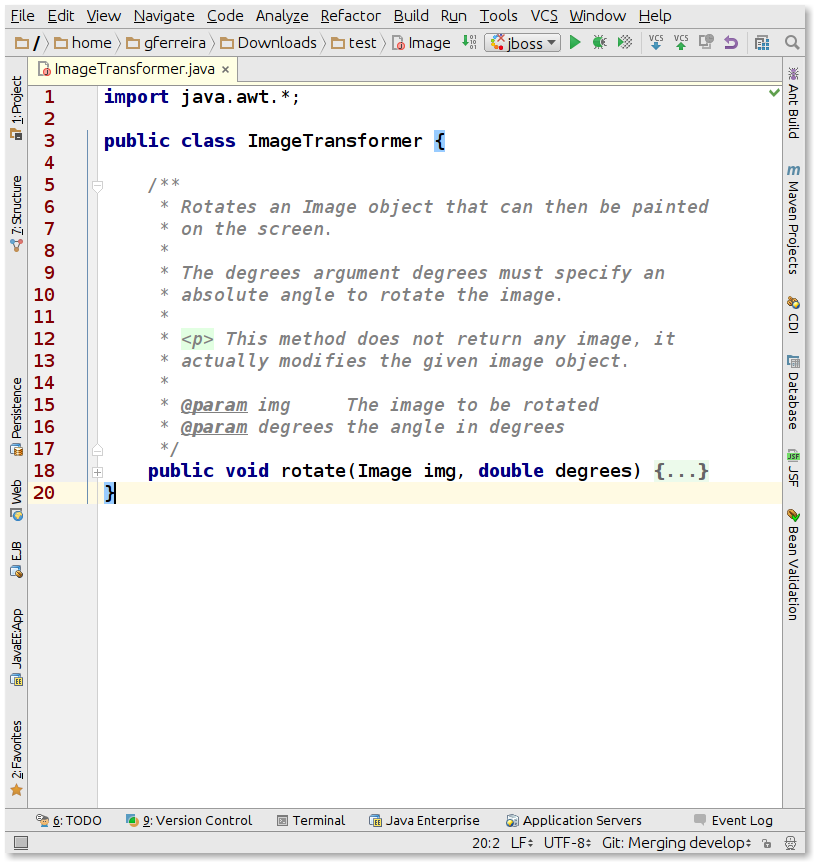
\includegraphics[width=.9\linewidth]{images/javadoc-code}
  \caption{A Javadoc annotation of a Java method}
  \label{fig:javadoc-code}
\end{subfigure}%
\begin{subfigure}{.5\textwidth}
  \centering
  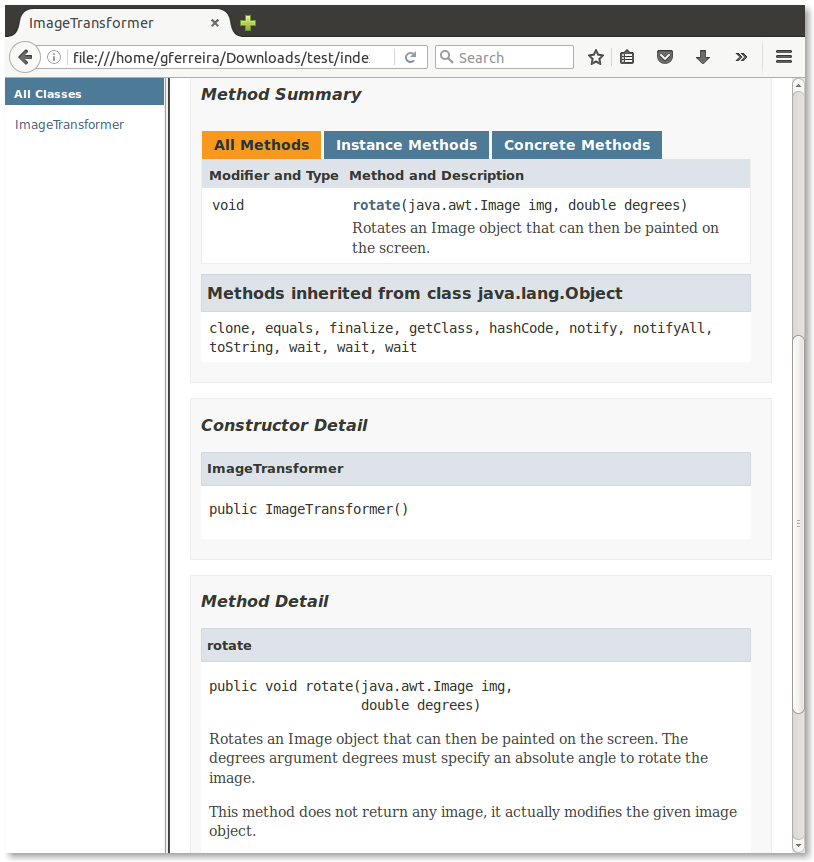
\includegraphics[width=.9\linewidth]{images/javadoc}
  \caption{Javadoc HTML auto-generated}
  \label{fig:javadocgen}
\end{subfigure}
\caption{Javadoc generation of a HTML page from a documented Java method. In the left is the source code commented with the opening tag \texttt{/**}, in the right is the generated documentation page.}
\label{fig:javadoc}
\end{figure}

Figure~\ref{fig:javadoc} shows an example of Javadoc an industry standard tool which provides interesting functionalities for documenting Java classes. The HTML format keeps information together giving the convenience of being able to hyperlink related documentation. As a result, programmers can easily navigate through classes and their respective methods. Moreover, Javadoc provides a widely integration trough \glspl{ide} (e.g. Eclipse, IntelliJ, NetBeans, etc), being able to generate automatic comments and the proper documentation using these \glspl{ide}. This tool indeed helps to produce a presentable documentation without much effort, however there are clearly important points to improve.

In these tools, the documentation are essentially represented as rows of plain text. Despite of supporting HTML format for generating the final documentation, there is no rich media resource in the generated pages only text and hyperlinks to other pages. Moreover, the developer's attention is taken from code into a series of static pages that do not add more information, actually they show less than the source code. And the automatic comments generated by \glspl{ide} are useless comments that do not add any rigorous information for the developer (e.g. a method called \texttt{getFoo()} would be commented as ``This method gets a foo"). Finally, these tools are more focused on creating an industry standard documentation mainly devoted to the client, than focused on creating a useful documentation that effectively helps developers to comprehend the code and its architecture.

The representation of source code dramatically affects its comprehensibility and usability~\citep{baecker1986design}. The idea of enhancing program comprehension and usability by improving its representation using richer media resources is not new in the literature~\citep{marcus1982graphic,baecker1986design,baecker1983enhancing}. These researches define design principles for enhancing program visualization, showing the impact of those principles in the readability of the code. Based on these works, subsequently researches and implementations have been tried to keep those principles alive inside the academic context. For example Barista~\citep{ko2006barista} implements some of these principles  allowing media-rich annotation in the code editor (see Figure~\ref{fig:barista}), while Codelets~\citep{oney2012codelets} focus on supporting media-rich resources in code completion by enabling HTML icons visualization (see Figure~\ref{fig:codelet}) helping developer to write HTML pages 43\% faster than when using a standard Web browser\citep{oney2012codelets}.

\begin{figure}
\centering
\begin{subfigure}{.5\textwidth}
  \centering
  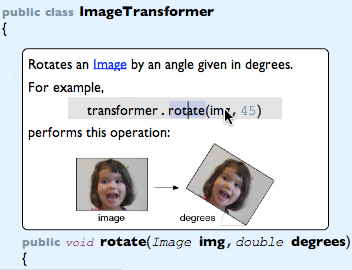
\includegraphics[width=.7\linewidth]{images/barista}
  \caption{A media-rich annotation in the Barista editor}
  \label{fig:barista}
\end{subfigure}%
\begin{subfigure}{.5\textwidth}
  \centering
  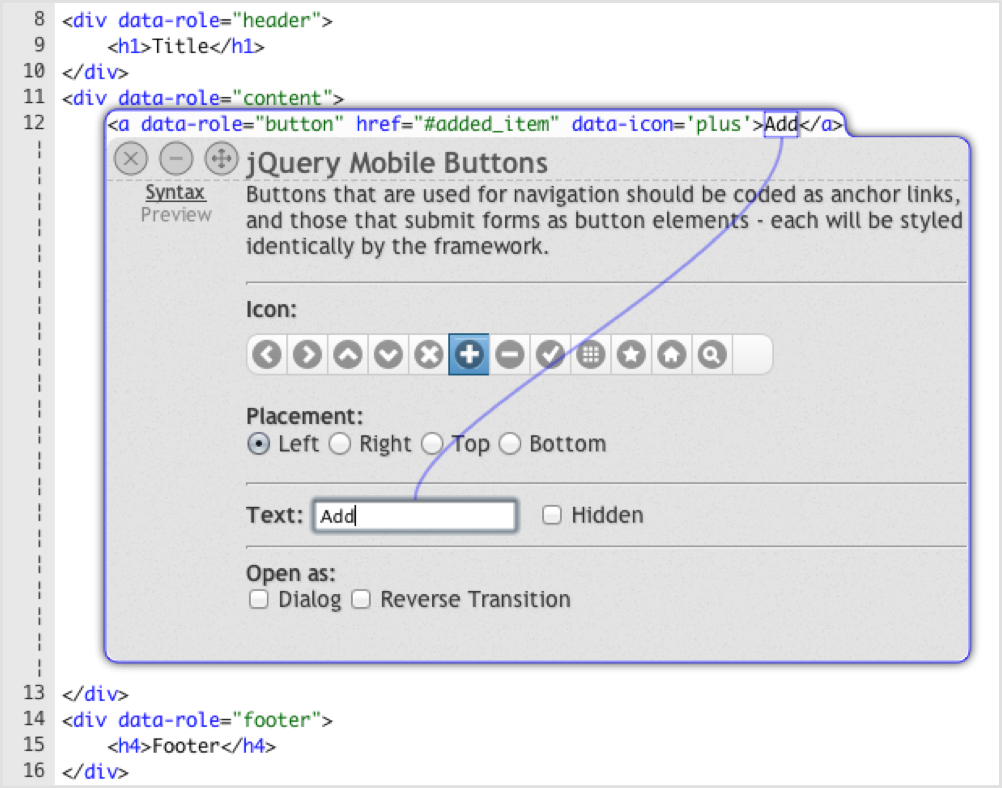
\includegraphics[width=.7\linewidth]{images/codelet}
  \caption{A Codelet inline helper}
  \label{fig:codelet}
\end{subfigure}
\caption{Example of media-rich annotations supported by code editors. On the left is Barista editor showing a Java method with richer annotations including images. On the right is the Codelets implementation showing the inline helper with icons defined for mobile buttons.}
\label{fig:richmedia}
\end{figure}

Barista~(Figure~\ref{fig:barista}) proposes a framework for creating interactive tools. It is build on top of Citrus~\citep{ko2005citrus}, a programming language intentionally created for supporting the creation of structured editors, consequently it is a positive factor that facilitates the implementation of the proposed tools. These tools implement several principles of usability and readability, for example media-rich annotation of methods (including hyperlink and diagrams inside the comments; allowing show/dismiss the comments by double clicking), readable pretty-printed view of formulas (enabling edit of these expressions by double clicking), and so on. However Barista seams to be more a prove of concept, than actually a system used nowadays, besides the programming language used in this implementation be probably obsolete. On the other hand, Codelets~(Figure~\ref{fig:codelet}) uses media-rich resources to present in a pop-up a variety of icons that develops can choose to create their web pages. However it is more related with code completion technologies than properly support program documentation.

The lack of tools that properly document a program is still a problem that negatively affects the \gls{gd} area. There is no such a tool which properly documents a program or automates the process of documentation. However the implementation of this tool and many other potentially useful tools are difficult or impossible in programming environments like DesignScript~\citep{aish2012designscript}, Monkey (and other textual environments used in \gls{gd}) that visually represent source code as rows of plain text. In the other hand, the visual programming languages, supported by environments such as Grasshopper and Dynamo, represent the source code visually with boxes and lines. However, to document these visual programming languages usually a box of plain text are provided, so that users can place it any where at program. As a result, the program documentation becomes spread in a bunch of boxes randomly placed around the program components, clearly an avoidable way to document a program.

This problem is aggravated by the increasing use of \gls{gd} methods to support the design and conception of real architectural projects. The architectural projects, in the likeness of software projects, has a design phase where architects study the problem which they want to solve, analyze eventual constraints imposed by the client or even by external factors, and then define a draft of the solution. At the end of this process several artifacts are produced, is commonly expected diagrams and handmade sketches (as those portrayed in Figure~\ref{fig:sketch-fig}). These sketches are commonly used among architects since early days of architecture~\citep{do2001thinking}, because they represent a compact medium to convey complex ideas. The information generated in the design phase can be sufficient enough to model and construct the entire project serving as a start point, and a basis, to develop the project. 

For example, the Figure~\ref{fig:sketch-using} (reference here) shows the importance of this phase in the architectural conception. In this example the architect started by drawing a series of  sketches annotating them with dimensional and spacial parameters such as height ($h$), diameter ($d$), the normal vector ($\vec{N}$), and vertex points (e.g. $P_0, P_1, P_2, ...$) of each shape (see Figure~\ref{fig:sketch-fig}). Then he used those shapes, as a small piece of design, by combining them to create a distinct pattern. After, he used this pattern by applying it into a 2D sinusoidal surface which represents the ceiling of a geometric structure, as shown in Figure~\ref{fig:sketch-fig-result}. In this example is also clear the known approach in software engineering: dive to conquer, because the architect started by designing the small pieces of the model and then he combined those unities of design to project the final structure. Each piece was carefully designed to join with the whole model, it is important to understand what is the meaning of those annotations to realize how can I propose a useful tool that effectively helps in the program documentation.

\begin{figure}
\centering
\begin{subfigure}{.6\textwidth}
  \centering
  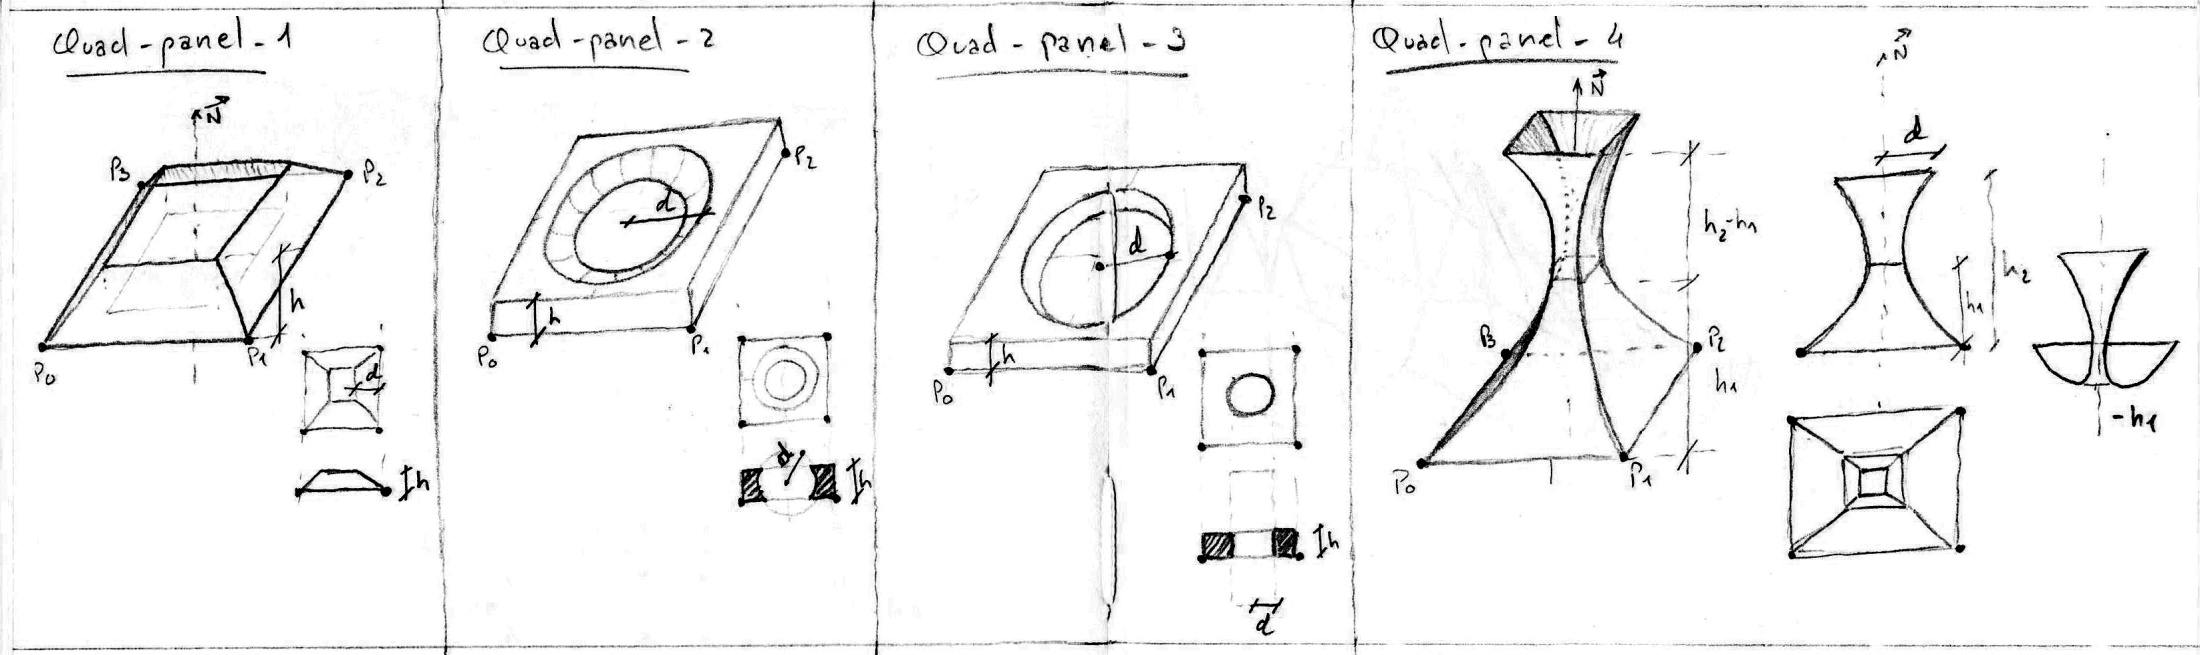
\includegraphics[width=.95\linewidth]{images/real-sketch}
  \caption{Sketches made during architectural design phase}
  \label{fig:sketch-fig}
\end{subfigure}%
\begin{subfigure}{.4\textwidth}
  \centering
  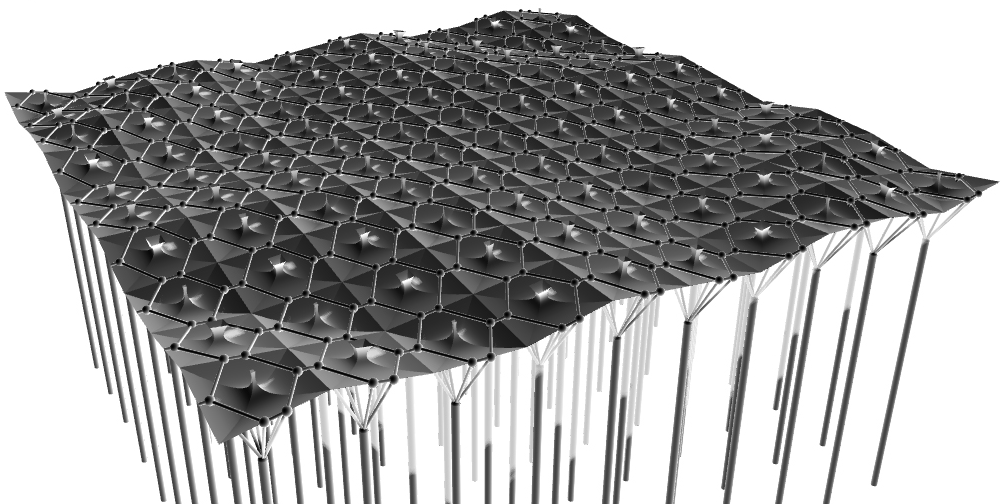
\includegraphics[width=1.0\linewidth]{images/real-sketch-result1}
  \caption{An application of the objects modeled previously in an architectural model}
  \label{fig:sketch-fig-result}
\end{subfigure}
\caption{Typical example showing the importance of design phase in the geometric model conception}
\label{fig:sketch-using}
\end{figure}

In the context of \gls{gd} methods these sketches becomes even more relevant because they serve as basis for implementing the program. By definition of \gls{gd} method it formally defines a description of an architectural model~\citep{mccormack2004generative}. In this way, while the code define the geometric object textually, the sketch define the geometric object visually. Consequently, it is fundamental during the development of the program but it is also a rich source for documenting the program. Different from the typical programs in software engineering which is purely textual and may express concepts that is difficult or even impossible to represent graphically, the program in \gls{gd} has this particularity of being able to represent its concepts through sketches or diagrams.

Surely sketches and diagrams are a suitable medium to express complex ideas. More than that, the architect frequently uses sketches because it helps him to reason about the conception of the design itself. And the \gls{gd} approach does not change this fact, on the contrary the use of sketch to illustrate program's components become even more popular, because it turns programming into a more  concrete and noticeable task, giving special clues for novice programmers. At the end of writing the program, all architect's decisions and insightful design, applied to construct the final program, are encapsulated in these sketches. As a result, these
sketches are also an essential artifact to comprehend the program specially after its release. 

For example consider the Figure~\ref{fig:chairseat} (reference here) that portrays a real example of a chair seat which was parametrically modeled. Even the less curious reader will wonder to know what each symbol of this image means. Some of them are more obvious than others, for instance the angles and the differences between them, however this diagram has its meaning embedded in problem context. It means that, those symbols in the image are variables which were created purposely to solve the problem of creating different shape of seats by varying the variable values. So the sketch proposes a parametric model of chair seats, additionally it contextualizes the meaning of each variable. Using this example the architect is able to create a suitable \gls{gd} method that creates this chair seat, however the \gls{gd} approach is not so straightforward as it seems to be. 

\begin{figure}[!htbp]
%\vspace{-5pt}
  \centering
  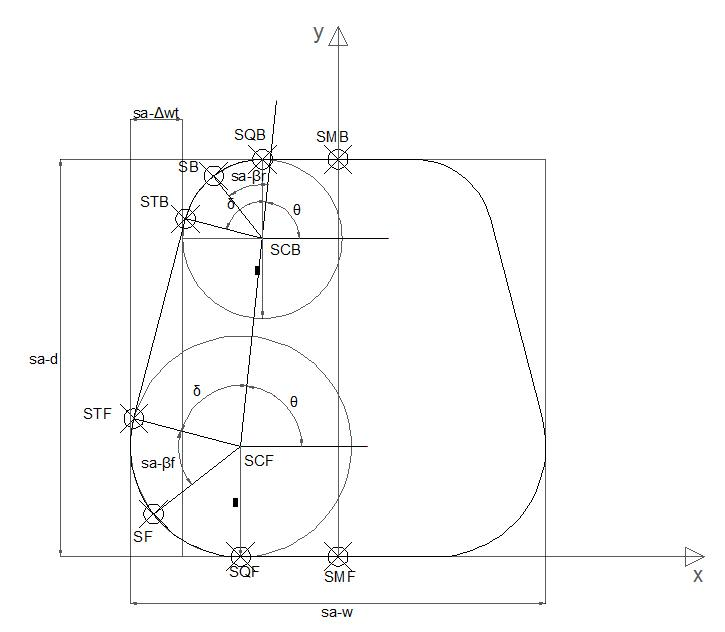
\includegraphics[width=0.5\textwidth]{images/seat}
    %\vspace{-15pt}
    \caption{A real sketch of a chair seat. In this sketch the seat is parametrized with some geometric variables. Some of them are intuitively noticeable, e.g. the angle symbols $\delta$, $\theta$, and $\beta$, but rest of them are not, because they have its meaning embedded in the problem context}
    %\vspace{-5pt}  
  \label{fig:chairseat}
\end{figure}

The problem with the \gls{gd} methods is that when a geometric model is rewritten in a programming language all visual information that perhaps its diagrams show is lost. For example the diagram in Figure~\ref{fig:chairseat} would be written using the following function signature: \\

\begin{minipage}[c]{.8\textwidth}
\texttt{/* this function creates a chair seat */} \\
\texttt{make-seat(SMF, SCF, SCB, sa-d, sa-w, sa-$\Delta$wt, sa-$\beta$r, sa-$\beta$f) \{} \\
\texttt{\hphantom{...} // the function body} \\
\qquad \texttt{\hphantom{...} ...} \\
\texttt{\}}
\end{minipage} \\

For the architect who did the sketch and implemented the code this function may appear simple enough to be understood. For people who will get this code posteriorly this kind of functions could give a headache nonetheless. Actually in the architect's mind all these functions parameters make sense, because they all are part of the design and the sketch can prove it. The problem is that the sketch is not delivered with the program, moreover the program is usually delivered without any documentation or may have useless comments as that one in the example. Consequently, it negatively affects people who need to use this program, because without documentation they cannot understand the program well enough to use, or modify it, affecting the entire \gls{gd} community. 

\section{Sketch-program correlation tool}

As discussed in the previous section, the lack of documentation in \gls{gd} programs affects negatively its users. In fact this problem is beyond \gls{gd} area, it affects also the field of software engineering. In this field, there were attempts to improve this problem by improving the quality of program documentation, most prominently, \textit{literate programming}~\citep{knuth1984literate}. This work proposed a programming paradigm that promoted the fact that program are written for people first and foremost, and that documentation should be emphasized just as much as code. Unfortunately, these attempts did not reach the intended goals, mainly because writing good documentation takes considerable amount of time and effort.

A more recent work~\citep{learnableProg} suggested that the programming environment should minimize this tough work required to write documentation by providing the documentation programmers need when they are reading the code. In this work, Victor outlines the following idea:

\blockquote{The environment is responsible for making meaning transparent. The environment must enable the reader to effortlessly read the program, to decode the code, so he can concentrate on genuine programming concepts~\citep{learnableProg}}

Figure~\ref{fig:victor-ex} shows a prototype, presented with this work, that demonstrates how the environment can improve the program readability. The code in prototype is written in Processing language~\citep{Reas2006} (on the left) and it  sets the environment color to green and creates two geometric objects: a circle and rectangle (on the right) by using the Processing functions: \texttt{fill, ellipse and rect}. This programming environment make meaning of each element of the code transparent, by providing labels on mouse-over. For example, the reader will know that the fourth parameter of function \texttt{rect} will change the height of the rectangle when he points to that parameter. And he can also point to every element of this code to get its meaning, so even before he makes any change in this code he will know exactly what the code is doing.     

\begin{figure}[!htbp]
%\vspace{-5pt}
  \centering
  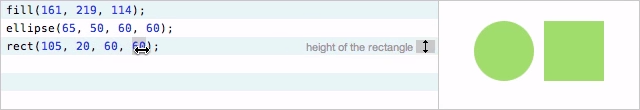
\includegraphics[width=.7\textwidth]{images/victor-example}
    %\vspace{-15pt}
    \caption{A programming environment that helps in the program readability. On the right, is a sample of code, written in Processing language, that creates a green circle and rectangle. On the right, is the produced result of this code. Each element of this program, including the functions and its arguments, are labeled so when user point the mouse over an element its label appears on the editor.}
    %\vspace{-5pt}  
  \label{fig:victor-ex}
\end{figure}

Labeling the program elements on mouse-over indeed make the program meaning more explicit, but this technique does not replace the need of a proper documentation. The main problem with this approach is that these labeled functions already exist in Processing, so this feature is more intended to avoid unnecessary searches on the Processing manual, than alternatively provides a way to document the program. For any user defined function this feature will not work, consequently the programmer must take considerable amount of time and effort to create its own documentation.

The reality in architecture is quite different form that in software engineering: it is part of the design process to produce documentation in the form of sketches. This means that it is not necessary to write huge amounts of textual documentation to explain a \gls{gd} program. We only need to annotate the already existing sketches and combine them with the program, thus providing visual explanations of what the program is supposed to do.

In Figure~\ref{fig:sc-tool} I propose the \textit{sketch-program correlation tool} that shows how sketches and code can be combined to provide useful documentation for the programmer by using the sketches made in a early phase of program design. This example illustrates a function that draws an arrow giving the base point $P$, the direction $\alpha$, the height $\rho$, and the width $\beta$ and size $\sigma$ of the arrow tip. This information is all condensed in the sketch, maybe even more precise. So the idea of this tools is to take advantage of this fact by pointing out what is the meaning of each function parameter, found in the code, in the context of the sketch (and vice versa). In this way, when the user has the mouse over a function parameter he immediately sees what that parameter correspond in the sketch, and  the inverse is also valid: when he moves the mouse over a symbol in the image he immediately see its meaning in the code. That helps him to create a mental model of the program even before to change it.

\begin{figure}[!htbp]
%\vspace{-5pt}
  \centering
  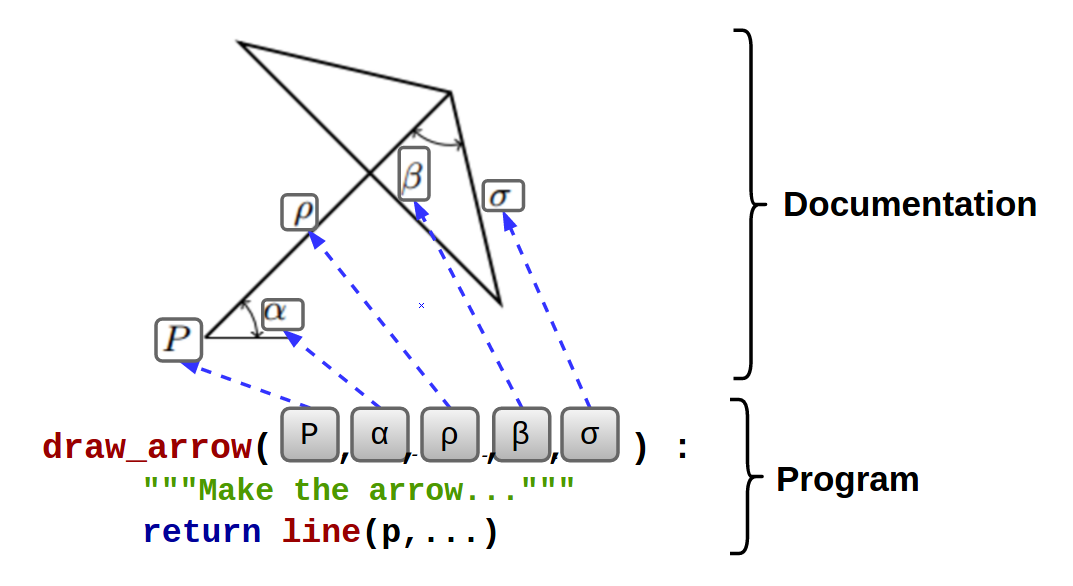
\includegraphics[width=0.5\textwidth]{images/proposed-sc-tool}
    %\vspace{-15pt}
    \caption{\textit{Sketch-program correlation tool} showing how to combine fragments of the program with sketches. In this example all the function parameters has a correspondent symbol in the sketch that illustrate its meaning}
    %\vspace{-5pt}  
  \label{fig:sc-tool}
\end{figure}

As demonstrated in early works, the underline principle behind this tool can in fact helps in the program readability, consequently helping in the overall process of program comprehensibility. However implement this tool in the current environments for \gls{gd} is undoubtedly a hard  challenge, due the absence of certain capabilities required for implementing this kind of tool considering the current state of \gls{gd} environments.

Perhaps the first challenge imposed by this tool, is in how to include images in the code editor. It seems a trivial problem, however the possibility to insert a simple image in the code editor is unsupportable for at least the majority of code editors. Specially in \gls{gd} where the environments used for textual languages generally only support rows of plain text. Until the time we are not aware of any other code editors that provide such a capability, in exception of Rosetta tool~\citep{lopes2011portable} that provides an enhanced code editor that supports images and other media-rich elements, by using DrRacket~\citep{findler2002drscheme} as its code editor.

A inherent concern in the fact of supporting images in the code editor is on how to store it. The strategy used by DrRacket, is to serialize the image and store it in ascii-encoded binary format. The problem of this strategy is that once the programmer inserts an image in his code and save it, he will not be able to change its code again using other text editor. So this method does not provide any backwards-compatibility with other text editors potentially useful to write programs. As a result, it makes difficult, or even impossible, the portability of the program among those different text editors.

I propose another approach to this problem that assures backwards-compatability. The first step is to define a standard annotation that will be used to include the image, similarly to the Java doc annotation. Then requires the use of that annotation upon an event of image insertion. Thus to include an image the programmer should quote the image with that annotation, as the example depicted in Figure~\ref{fig:inline-image}. As a result, it will be possible for the program environment to distinguish images from source code and proceed to an adequate treatment for those images. 

\begin{figure}[!htbp]
%\vspace{-5pt}
  \centering
  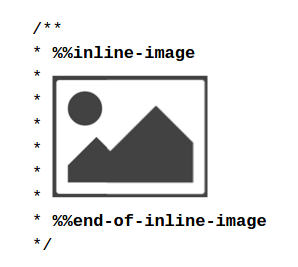
\includegraphics[width=.25\textwidth]{images/inline-image-example}
    %\vspace{-15pt}
    \caption{Example of inline-image annotation.}
    %\vspace{-5pt}  
  \label{fig:inline-image}
\end{figure}

By using this convention, when the programmer save his code all images under that annotation can be stored as a simple source code comment. For example considering the annotation showed in Figure~\ref{fig:inline-image}, the following string would be generated by parsing that annotation:

\begin{center}
\begin{minipage}[c]{.6\textwidth}
\texttt{// \%\%image \$\{USER\_HOME\}/project/sketch1.jpg \%\%}
\end{minipage} \\
\end{center}

The above text is a convection that represents the relative path from where the code editor loaded the image. In this way if the code editor cannot resolve this path and find the image, the code could be showed anyway by displaying just that comment, thus the code can be opened in any text editor. Of course to be able to see the images, programmers must open the code in the text editor capable to interpret that annotations and display the images. 

Other systems, to avoid the problem of incompatibility among editors convert the code into a textual format, for example Barista~\citep{ko2006barista} saves the code in XML. However the presented approach goes further, because it does not impose any language specific requirement, the code is stored as it is (ordinary plain text). So it is up to the code editor to implement suitable methods to show the images.

Nevertheless, an interesting challenge imposed by the sketch-program correlation tool is the automatic recognition of text and symbols in images. Fortunately, this is an old problem which is part of the ancient dream of replicating the human functions by machines, making the machine able to perform tasks like reading. To concertize this dream was realized that information should be readable both to humans and to machine and alternative inputs can not be predefined. As consequence of this probably inputs, an \gls{ocr} system would be necessary for dealing with the problem of recognizing optically processed characters. Optical recognition is performed after the writing or printing has been completed. Therefore the idea of this system is avoiding the traditional way of entering data into a computer through the keyboard by providing a more efficient way for it.

The \gls{ocr} systems rapidly became a prominent field of study that gave substantial incentives for making pattern recognition and image analysis matured fields of science. The very first attempts can actually be found back in 1870~\citep{eikvil1993optical} with the retina scanner which was an image transmission system using a mosaic of photocells. From then, consecutive attempts were made to improve the methods of \gls{ocr} systems, specially by sophisticating the retina scanner and creating OCR machines that became commercially available in the 1950's. Posteriorly, HP as a possible software and/or hardware add-on for HP's line of flatbed scanners, proposed a novel open-source project: Tesseract~\citep{smith2007overview} OCR engine. This project was then sponsored by Google and nowadays is one of the most accurate OCR engine on the market used widely in several web applications.

Clearly the subject of character recognition is extremely extensive and its details are beyond the scope of this dissertation. However, to propose my solution of recognizing automatically text in image, I based on the functionality of the \gls{ocr} engine, namely the Tesseract~\citep{smith2007overview}, that accepts an image file and returns a file with the recognized characters and their respective coordinates on the image. However, the Tesseract is a local application that needs to be installed in the user's computer, or be included as external libraries on the program, which may affect the portability of the application and its use.

To solve this problem I propose the use of \gls{ocr} Web Service, such as\footnote{\texttt{http://www.onlineocr.net/}},\footnote{\texttt{http://www.free-ocr.com/}} that provides the same functionality, because they are build on top of Tesseract, but it defines a more standardized way for integrating the applications using the SOAP or REST. Figure~\ref{fig:sc-tool-arch} shows the architecture of this tool. 


\begin{figure}[!htbp]
%\vspace{-5pt}
  \centering
  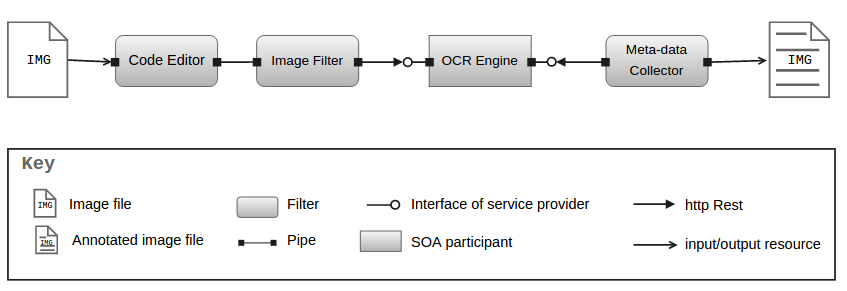
\includegraphics[width=.7\textwidth]{images/sc-tool-architecture}
    %\vspace{-15pt}
    \caption{Data flow view combining two styles: pipe-and-filter style and client-server style.}
    %\vspace{-5pt}  
  \label{fig:sc-tool-arch}
\end{figure}